\documentclass [a4paper]{article}
%% Language and font encoding
\usepackage[english]{babel}
\usepackage[utf8x]{inputenc}
\usepackage[T1]{fontenc}
\usepackage{gentium}


%% sets page sizes and margins
\usepackage[a4paper,top=1cm,right=3cm,bottom=2cm,left=3cm]{geometry}

%% useful packages
\usepackage{amsmath}
\usepackage{amssymb}
\usepackage{graphicx}
\usepackage[colorinlistoftodos]{todonotes}
\usepackage[colorlinks=true,allcolors=blue]{hyperref}
\usepackage{color}
\usepackage{textcomp}
\definecolor{light-gray}{rgb}{0.8,0.8,0.8}
\usepackage[singlespacing]{setspace}
\usepackage{array}
\usepackage{ragged2e}
\usepackage{tikz}
\usepackage{scalerel,stackengine}

%header and footer
\usepackage{fancyhdr}
\pagestyle{fancy}
\fancyhead
\fancyfoot
\renewcommand{\headrulewidth}{0pt}
%
\title{book_n.text}

\begin{document}
\pagestyle{fancy}
\begin{flushleft}
\section*{\Huge\textbf{4}}
\vspace*{0.5cm}
{\Huge\textbf{Pictorial proofs}}\\
\end{flushleft}
\vspace*{3cm}
\begin{justify}
\colorbox{light-gray}{\begin{minipage}{\textwidth}
\begin{tabular}{l r}
\large 4.1 Adding odd numbers \hspace{10cm} 58 \\
\large 4.2 Arithmetic and geometric means \hspace{7.9cm} 60 \\
\large 4.3 Approximating the logarithm \hspace{8.5cm} 66 \\
\large 4.4 Bisecting a triangle \hspace{ 10.3cm}  70\\
\large 4.5 Summing series \hspace{10.9cm} 73 \\
\large 4.6 \textit{Summary and further problems} \hspace{8.7cm} 75\\
\end{tabular}
\end{minipage}}
\end{justify}

\vspace*{5mm}
\pagestyle{fancy}
\begin{justify}
\Large Have you ever worked through a proof, understood and confirmed each step,yet not believed the theorem? You realize \textit{that} the theorem is true, but not \textit{why} it is true.\\
\vspace*{0.02mm}\\
To see some contrast in a familiar example, imagine learning that your child has a fever and hearing the temperature in Fahrenheit or Celsius degrees, whichever is less familiar. In my everyday experience, temperatures are mostly Fahrenheit. When I hear about a temperature of 40\textdegree C, I therefore react in two stages:\\ 
\vspace*{2mm}\\
1. I convert 40\textdegree \ C to Fahrenheit: 40 \texttimes \ 1.8 + 33 = 104.\\
\vspace*{0.02mm}\\
2. I react: "Wow, 104\textdegree \ F. That's dangerous! Get thee to a doctor!"\\
\vspace*{0.02mm}\\
The Celsius temperature, although symbolically equivalent to the Fahrenheit temperature, elicits no reaction. My danger sense activates only after the temperature conversion connects the temperature to my experience.\\
\vspace*{0.02mm}\\
A symbolic description, whether a proof or an unfamiliar temperature, is unconvincing compared to an argument that speaks to our perpetual system. The reason lies in how our brains acquired the capacity for symbolic reasoning. (See \textit{Evolving Brains} [2] for an illustrated,scholarly history of the brain.) Symbolic, sequential reasoning requires language, which has
\end{justify}


\newpage
\pagestyle{fancy}
\begin{justify}
\Large{\textbf{58}} \hspace{11.3cm} \large{\textit{4 Pictorial proofs}}\\
\vspace*{0.4cm}\\
\Large evolved for only $10^5$ yeah.Although $10^5$ spans many human lifetimes,it is an evolutionary eyeblink. In particular, it is short and compared to the time span over which our perceptual hardware has evolved: For several hundred million years,organisms have refined their capacities for hearing, smelling, tasting and seeing.\\

\vspace*{2mm}
\noindent Evolution has worked 1000 times longer on our perceptual abilities than our own symbolic-reasoning abilities.Compared to our perceptual hardware, our symbolic, sequential hardware ill-developed latecomer. Not surprisingly,our perceptual abilities far surpass our symbolic abilities.Even an apparently high-level symbolic ability such as playing grandmaster chess uses mostly perceptual hardware [16]. \textit{seeing} an idea conveys to us a depth of understanding that a symbolic description of it cannot easily match.\\
\vspace*{0.5mm}\\
\colorbox{light-gray}{\begin{minipage}{\textwidth}
\begin{justify}
\textbf{\hspace*{3mm} \large Problem 4.1} \hspace{3mm} \textbf{ \large Computers versus people}\\
\hspace{2cm} \large \hspace*{3mm} At tasks like expanding $(x + 2y)^{50}$, computers are much faster than people. At tasks \hspace*{3mm} like recognizing faces or smells, even young children are much faster than current \hspace*{3mm} computers. How do you explain these contrasts?
\vspace*{2mm}\\
\textbf{\hspace*{3mm} \large Problem 4.2} \hspace{3mm} \textbf{ \large Linguistic evidence for the importance of perception}\\
\large \hspace*{3mm} In your favorite language(s), think of the many synonyms for understanding (for \hspace*{4.25mm} example, grasp).
\end{justify}
\end{minipage}
}
\end{justify}
\vspace*{2mm}
\hspace{-3em{\LARGE{\textbf{4.1 Adding odd numbers}}}}
\vspace{0.2mm}\\
\begin{justify}
\Large To illustrate the value of pictures, let's find the sum of the first \textit{n} odd numbers (also the subject of Problem 2.25):
\end{justify}
\Large \[ \hspace*{2em} S_n = \underbrace{1 + 3 + 5 + . . . +
(2n - 1)}_\text{\Large\textit{n} terms}. \hspace{60mm} (4.1)\]
\begin{justify}
\Large Easy cases such as $n = 1$, 2, or 3 lead to the conjecture that $S_n = n^2$. But how can the conjucture be proved? The standard symbolic method is proof by induction:
\vspace*{2mm}\\
\noindent 1.
Verify the $S_n = n^2$ for the \textit{base case} $n = 1$. In that case, $S_1$ is 1, as is \hspace*{1em} $n^2$, so the base case is verified.
\vspace*{2mm}\\
\noindent 2. Make the \textit{induction hypothesis:} Assume that $S_m = m^2$ for \textit{m} less than \hspace*{0.9em} equal to a maximum value \textit{n}. For this proof, the following, weaker \hspace*{1.2em}induction hypothesis is sufficient:
\end{justify}
\newpage
\pagestyle{fancy}
\begin{justify}
\Large {\textit{\hspace*{-2em}4.1 \hspace*{1mm} Adding odd numbers} \hspace{10cm} \textbf{59}}
\end{justify}
\vspace*{3mm}
$$\hspace*{2em} \sum_{1}^{n}{(2k-1) = n^2.\hspace*{9.35cm} (4.2)}$$
\vspace*{3mm}
\begin{justify}
\Large In other words, we assume the theorem only in the case that $m=n$.\\
\hspace*{-1.5em}3. Perform the \textit{induction step:} Use the induction hypothesis to show that $S_{n+1} = (n + 1)^2$. The sum $S_{n+1}$ splits into two pieces:
\end{justify}
$$\hspace*{2em} S_{n+1} = \sum_{1}^{n+1}{(2r-1)} = (2n + 1) + \sum_{1}^{n}{(2k-1). \hspace*{3.7cm} (4.3)}$$
\begin{justify}
Thanks to the induction hypothesis, the sum on the right is $n^2$. Thus
\end{justify}
$$\hspace*{2em} S_{n+1} = (2n+1) + n^2, \hspace*{9cm} (4.4)$$
\begin{justify}
which is the $(n + 1)^2;$ and the theorem is proved.
\end{justify}
\begin{justify}
\hspace*{-1.5em} Although these steps prove the theorem, \textit{why} the sum $S_n$ ends up as $n^2$\\ \hspace*{-1.5em} still feels elusive.
\end{justify}
\begin{justify} \hspace*{-1.5em} That missing understanding\textemdash the kind of gestalt insight described by\\ \hspace*{-1.5em} Wertheimer [48]\textemdash requires a pictorial proof. Start by drawing each odd\\ \hspace*{-1.5em} number as an L-shaped puzzle piece:\\

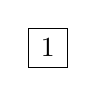
\begin{tikzpicture}
\draw (0,0) -- (0.5,0) -- (0.5,0.5) -- (0,0.5) -- cycle;
\node at (0.25,0.25){1};
\end{tikzpicture}
\hspace*{10mm}
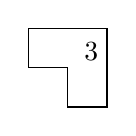
\begin{tikzpicture}
\draw (0,0) -- (0.5,0) -- (0.5,1) -- (-0.5,1) -- (-0.5,0.5) -- (0,0.5) -- cycle;
\node at (0.3,0.7){3};
\end{tikzpicture}
\hspace*{10mm}
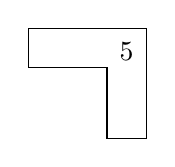
\begin{tikzpicture}
\draw (0,0) -- (0.5,0) -- (0.5,1.4) -- (-1,1.4) -- (-1,0.9) -- (0,0.9) -- cycle;
\node at (0.25,1.1) {5};
\end{tikzpicture}
\hspace*{8.5cm}(4.5)\\

\hspace*{-2.5em} \textit{How do these pieces fit together?}\\

\hspace*{-2.5em} Then compute $S_n$ by fitting together the puzzle pieces as follows:\\

$S_2$ \hspace*{3mm} = \hspace*{3mm} 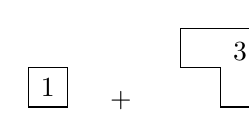
\begin{tikzpicture}
\draw (0,0) -- (0.5,0) -- (0.5,0.5) -- (0,0.5) -- cycle;
\node at (0.25,0.25){1};
\end {tikzpicture} \hspace*{3mm} + \begin{tikzpicture} \hspace*{5mm} \draw (0,0) -- (0.5,0) -- (0.5,1) -- (-0.5,1) -- (-0.5,0.5) -- (0,0.5) -- cycle;
\node at (0.25,0.7) {3};
\end{tikzpicture} \hspace*{4cm} = 
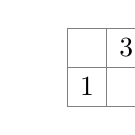
\begin{tikzpicture}
\hspace*{0.5cm}
\draw[step=5mm,gray,very thin] (-0.5,-0.5) grid (0.5,0.5);
\node at (-0.25,-0.25) {1};
\node at (0.25,0.25) {3};
\end{tikzpicture} \\

$S_3$ \hspace*{5mm} = \hspace*{3mm}
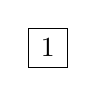
\begin{tikzpicture}
\draw (0,0) -- (0.5,0) -- (0.5,0.5) -- (0,0.5) -- cycle;
\node at (0.25,0.25){1};
\end{tikzpicture} \hspace*{4mm} +
\begin{tikzpicture} \hspace*{7mm}
\draw (0,0) -- (0.5,0) -- (0.5,1) -- (-0.5,1) -- (-0.5,0.5) -- (0,0.5) -- cycle;
\node at (0.25,0.7){3};
\end{tikzpicture} \hspace*{1.2cm} +
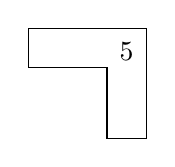
\begin{tikzpicture}
\draw (0,0) -- (0.5,0) -- (0.5,1.4) -- (-1,1.4) -- (-1,0.9) -- (0,0.9) -- cycle;
\node at (0.25,1.1){5};
\end{tikzpicture}
\hspace*{1cm} =
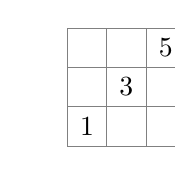
\begin{tikzpicture}
\hspace*{5mm}
\draw[step=5mm,gray,very thin]
(-0.5,-0.5) grid (1,1);
\node at (-0.25,-0.25){1};
\node at (0.25,0.25){3};
\node at (0.75,0.75){5};
\end{tikzpicture} \hspace*{4cm} (4.6)\\

\noindent Each successive odd number \textemdash each piece \textemdash extends the square by 1 unit in height and width, so the \textit{n} terms build an \textit{n} \texttimes \ \textit{n} square. [Or is it an\\ ($n-$1) \texttimes \ \ ($n-$1) square?] Therefore, their sum is $n^2$. After grasping this pictorial proof, you cannot forget why adding up the first \textit{n} odd numbers produces $n^2$.
\end{justify}

\newpage
\pagestyle{fancy}
\begin{justify}
\Large{\textbf{60}}  \hspace{11.3cm} \large{\textit{Pictorial proofs}}\\
\vspace*{0.5mm}\\
\colorbox{light-gray}
{\begin{minipage}{\textwidth}
\begin{justify}
\vspace*{3mm}
\large\textbf{\hspace{5mm} Problem 4.3} \hspace*{5mm} \large\textbf{Triangular numbers}\\

\noindent \hspace{0.5cm} Draw a picture or pictures to show that\\

$\hspace*{1cm} 1+2+3+...\textit{n}+ 3+2+1= n^2$ \hspace*{6cm} (4.7)\\

\noindent \hspace*{0.5cm} Then show that\\
$$\hspace{1cm} 1+2+3+... +n=\frac{n(n+1)}{2} \hspace*{6.5cm} (4.8)$$ 

\large\textbf Problem 4.4 \hspace*{5mm} \large\textbf{Three dimensions}\\

Draw a picture to show that\\
$$\hspace*{1cm} \sum _{0}^{n}{(2k^2+3k+1)=(n+1)^3} \hspace*{6.5cm}(4.9)$$\\
\hspace*{5mm} Give pictorial explanations for the 1 in the summand 3k$^2$ + 3k +1; for the 3 and the \hspace*{0.5cm} k$^2$ in the 3k$^2$; and for the 3 and the k in 3k.
\vspace*{3mm}
\end{justify}
\end{minipage}}

\vspace*{1cm}
\hspace{-3em{\LARGE{\textbf{4.2 Arithmetic and geometric means}}}}\\
\begin{justify}
\Large The next pictorial proof starts with two  nonnegatve numbers \textemdash for example, 3 and 4 \textemdash and compares the following two averages:\\

arithmetic mean \ \ $\equiv \Large \frac {3 + 4}{2}= 3.5; \hspace*{7cm} (4.10)$\\

geometric mean \ \ $\approx \sqrt{3 \times 4} =3.464. \hspace*{6cm} (4.11)$\\

\noindent Try another pair of numbers \textemdash for example, 1 and 2. the arithmetic mean is 1.5; the geometric mean is $\sqrt{2} \approx 1.414.$ For both pairs, the geometric mean is smaller than the arithmetic mean. This patter is general; it is the famous arithmetic-mean-geometric-mean (AM-GM) inequality [18]:\\

$$\hspace{-10cm} \frac {a+b}{\smash{\underbrace{2}}} \ge \underbrace{\sqrt{ab}} . $$\\
\noindent (The inequality requires that a, b $\ge$ 0.)
\end{justify}
\colorbox{light-gray}
{\begin{minipage}{\textwidth}
\begin{justify}
\textbf{\hspace*{3mm} \large Problem 4.5} \hspace{3mm} \textbf{\large More numerical examples}\\
\large \hspace*{3mm} the AM-GM inequality using varied numerical examples. What do you notice when \textit{a} \hspace*{3mm} and \textit{b} are close to each other? can you formalize the pattern? (See also Problem 4.16)
\end{justify}
\end{minipage}}
\end{justify}
\end{document}
